% !TEX program = pdflatex
% =====================================================================
%  TwA Teaching Webinar — Emily's full hour (~60 min)
%  June 17, 2026.
%  Master file — edit directly, do not reassemble.
%  Structure:
%    0. Welcome + housekeeping + audience + today's arc
%    1. Foundations (~10-15 min, 4 slides)
%    Part 1: Student data and AI (~15 min)
%    Part 2: De-identification in Practice — grading demo (~20 min)
%    C. Handoff to Erkmen
% =====================================================================
\documentclass[aspectratio=169, 10pt]{beamer}

%% ============================================================
%% PACKAGES
%% ============================================================
\usepackage[T1]{fontenc}
\usepackage{lmodern}
\usepackage{graphicx}
\usepackage{booktabs}
\usepackage{array}
\usepackage{tabularx}
\usepackage{colortbl}
\usepackage{tikz}
\usetikzlibrary{positioning, calc, arrows.meta, shapes.geometric, fit, shadows}
\usepackage[most]{tcolorbox}
\usepackage{fontawesome5}
\usepackage{hyperref}
\usepackage{multicol}
\usepackage{xcolor}
\usepackage{textcomp}
\usepackage{pifont}

\graphicspath{{figures/}}

%% ============================================================
%% COLOR DEFINITIONS
%% ============================================================
\definecolor{UVMGreen}{HTML}{154734}
\definecolor{UVMGold}{HTML}{D4A84B}
\definecolor{SlateTeal}{HTML}{1B4D5C}
\definecolor{DeepCharcoal}{HTML}{2C3E50}
\definecolor{SoftCoral}{HTML}{C0534D}
\definecolor{CoolGray}{HTML}{8899A6}
\definecolor{PaleSage}{HTML}{EDF2F0}
\definecolor{LightGold}{HTML}{FDF6E3}
\definecolor{DarkSlate}{HTML}{0F2B36}
\definecolor{AccentBlue}{HTML}{3498DB}
\definecolor{GoGreen}{HTML}{2E7D52}

%% ============================================================
%% BEAMER THEME SETUP
%% ============================================================
\setbeamercolor{structure}{fg=SlateTeal}
\setbeamercolor{normal text}{fg=DeepCharcoal}
\setbeamercolor{frametitle}{fg=SlateTeal}
\setbeamercolor{title}{fg=SlateTeal}
\setbeamercolor{subtitle}{fg=UVMGold}
\setbeamercolor{author}{fg=DeepCharcoal}
\setbeamercolor{date}{fg=CoolGray}
\setbeamercolor{institute}{fg=CoolGray}
\setbeamercolor{footline}{fg=CoolGray}
\setbeamercolor{block title}{fg=white, bg=SlateTeal}
\setbeamercolor{block body}{bg=PaleSage}
\setbeamercolor{alerted text}{fg=SoftCoral}
\setbeamercolor{item}{fg=SlateTeal}
\setbeamercolor{subitem}{fg=CoolGray}

\setbeamerfont{title}{size=\Large, series=\bfseries}
\setbeamerfont{subtitle}{size=\normalsize}
\setbeamerfont{frametitle}{size=\large, series=\bfseries}
\setbeamerfont{footline}{size=\tiny}

\setbeamertemplate{navigation symbols}{}

\setbeamertemplate{frametitle}{%
  \vskip14pt%
  \nointerlineskip%
  {\usebeamerfont{frametitle}\usebeamercolor[fg]{frametitle}\insertframetitle\par}%
  \vskip2pt%
  {\color{UVMGold}\rule{\textwidth}{1.2pt}}%
  \vskip3pt%
}

\setbeamertemplate{footline}{%
  \begin{beamercolorbox}[wd=\paperwidth, ht=16pt, right, rightskip=1.5cm]{footline}%
    \usebeamerfont{footline}\insertframenumber\,/\,\inserttotalframenumber\vskip3pt%
  \end{beamercolorbox}%
}

\setbeamertemplate{itemize item}{\color{SlateTeal}\raisebox{0.15ex}{\small$\blacktriangleright$}}
\setbeamertemplate{itemize subitem}{\color{CoolGray}\raisebox{0.1ex}{\footnotesize$\bullet$}}

\tcbset{
  keybox/.style={
    colback=PaleSage, colframe=SlateTeal, boxrule=0.8pt, arc=3pt,
    left=6pt, right=6pt, top=4pt, bottom=4pt,
    fonttitle=\bfseries\small\color{white}, coltitle=white, colbacktitle=SlateTeal,
  },
  accentbox/.style={
    colback=LightGold, colframe=UVMGold, boxrule=0.8pt, arc=3pt,
    left=6pt, right=6pt, top=4pt, bottom=4pt,
  },
  quotebox/.style={
    colback=PaleSage, colframe=SlateTeal!50, boxrule=0.5pt, arc=2pt,
    left=8pt, right=8pt, top=4pt, bottom=4pt,
    borderline west={3pt}{0pt}{UVMGold},
  },
  dobox/.style={
    colback=GoGreen!8, colframe=GoGreen, boxrule=0.8pt, arc=3pt,
    left=6pt, right=6pt, top=3pt, bottom=3pt,
    fonttitle=\bfseries\small\color{white}, coltitle=white, colbacktitle=GoGreen,
  },
  dontbox/.style={
    colback=SoftCoral!8, colframe=SoftCoral, boxrule=0.8pt, arc=3pt,
    left=6pt, right=6pt, top=3pt, bottom=3pt,
    fonttitle=\bfseries\small\color{white}, coltitle=white, colbacktitle=SoftCoral,
  },
  coralbox/.style={
    colback=SoftCoral!8, colframe=SoftCoral, boxrule=0.8pt, arc=3pt,
    left=6pt, right=6pt, top=3pt, bottom=3pt,
    fonttitle=\bfseries\small\color{white}, coltitle=white, colbacktitle=SoftCoral,
  },
  pipelinebox/.style={
    colback=SlateTeal!8, colframe=SlateTeal, boxrule=0.8pt, arc=3pt,
    left=5pt, right=5pt, top=3pt, bottom=3pt,
    fonttitle=\bfseries\scriptsize\color{white}, coltitle=white, colbacktitle=SlateTeal,
  },
}

\newcommand{\cmcite}[1]{{\scriptsize\color{CoolGray}\textit{#1}}}

%% ============================================================
%% METADATA
%% ============================================================
\title{Thinking With Agents}
\subtitle{Webinar 2: AI for Teaching}
\author{Emily Beam \quad\&\quad Erkmen G. Aslim}
\institute{University of Vermont \;$\cdot$\; Department of Economics}
\date{June 17, 2026}

\begin{document}

%% ====== SLIDE 0: TITLE ======
{
\setbeamertemplate{footline}{}
\begin{frame}[plain]
\begin{tikzpicture}[remember picture, overlay]
  \fill[SlateTeal] (current page.north west) rectangle (current page.south east);
  \fill[UVMGold] ([yshift=0.3cm]current page.center -| current page.west) rectangle ([yshift=0.25cm]current page.center -| current page.east);
  \node[anchor=center, text=white, font=\fontsize{28}{34}\bfseries\selectfont]
    at ([yshift=2.2cm]current page.center) {Thinking With Agents};
  \node[anchor=center, text=UVMGold, font=\fontsize{15}{20}\selectfont]
    at ([yshift=1.2cm]current page.center) {Webinar 2: Agentic AI for Teaching};
  \node[anchor=center, text=white, font=\large\bfseries]
    at ([yshift=-0.6cm]current page.center) {Emily Beam \quad\&\quad Erkmen G. Aslim};
  \node[anchor=center, text=PaleSage, font=\normalsize]
    at ([yshift=-1.3cm]current page.center) {University of Vermont \;$\cdot$\; Department of Economics};
  \node[anchor=center, text=CoolGray!70!white, font=\small]
    at ([yshift=-2.2cm]current page.center) {June 17, 2026 \quad$\cdot$\quad Live Online};
  \node[text=white, opacity=0.04, font=\fontsize{100}{100}\selectfont, anchor=center, rotate=-15]
    at ([xshift=5cm, yshift=1.5cm]current page.center) {\faChalkboardTeacher};
\end{tikzpicture}
\end{frame}
}

%% ====== HOUSEKEEPING ======
\begin{frame}{Welcome! How this works}
\vskip2pt
\begin{columns}[T]
\begin{column}{0.48\textwidth}
\begin{tcolorbox}[keybox, title={\faComments\quad Questions}]
\small  Drop questions in the \textbf{Q\,\&\,A} --- we'll review as we go and raise them during Q\,\&\,A time
\end{tcolorbox}
\vskip4pt
\begin{tcolorbox}[keybox, title={\faVideo\quad Recording}]
\small We're \textbf{not} posting the full recording publicly --- but slides, skills, etc. will be posted on https://thinkingwithagents.github.io/
\end{tcolorbox}
\end{column}
\begin{column}{0.48\textwidth}
\vskip4pt
\begin{tcolorbox}[accentbox, top=3pt, bottom=3pt]
\small This is \textbf{mostly live}. Things may break --- that's part of the honest picture.
\end{tcolorbox}
\end{column}
\end{columns}
\end{frame}

%% ====== WHO'S IN THE ROOM ======
\begin{frame}{Who's in the room}
\vskip-8pt
{\small Or at least, who signed up}
\vskip-4pt
\begin{center}
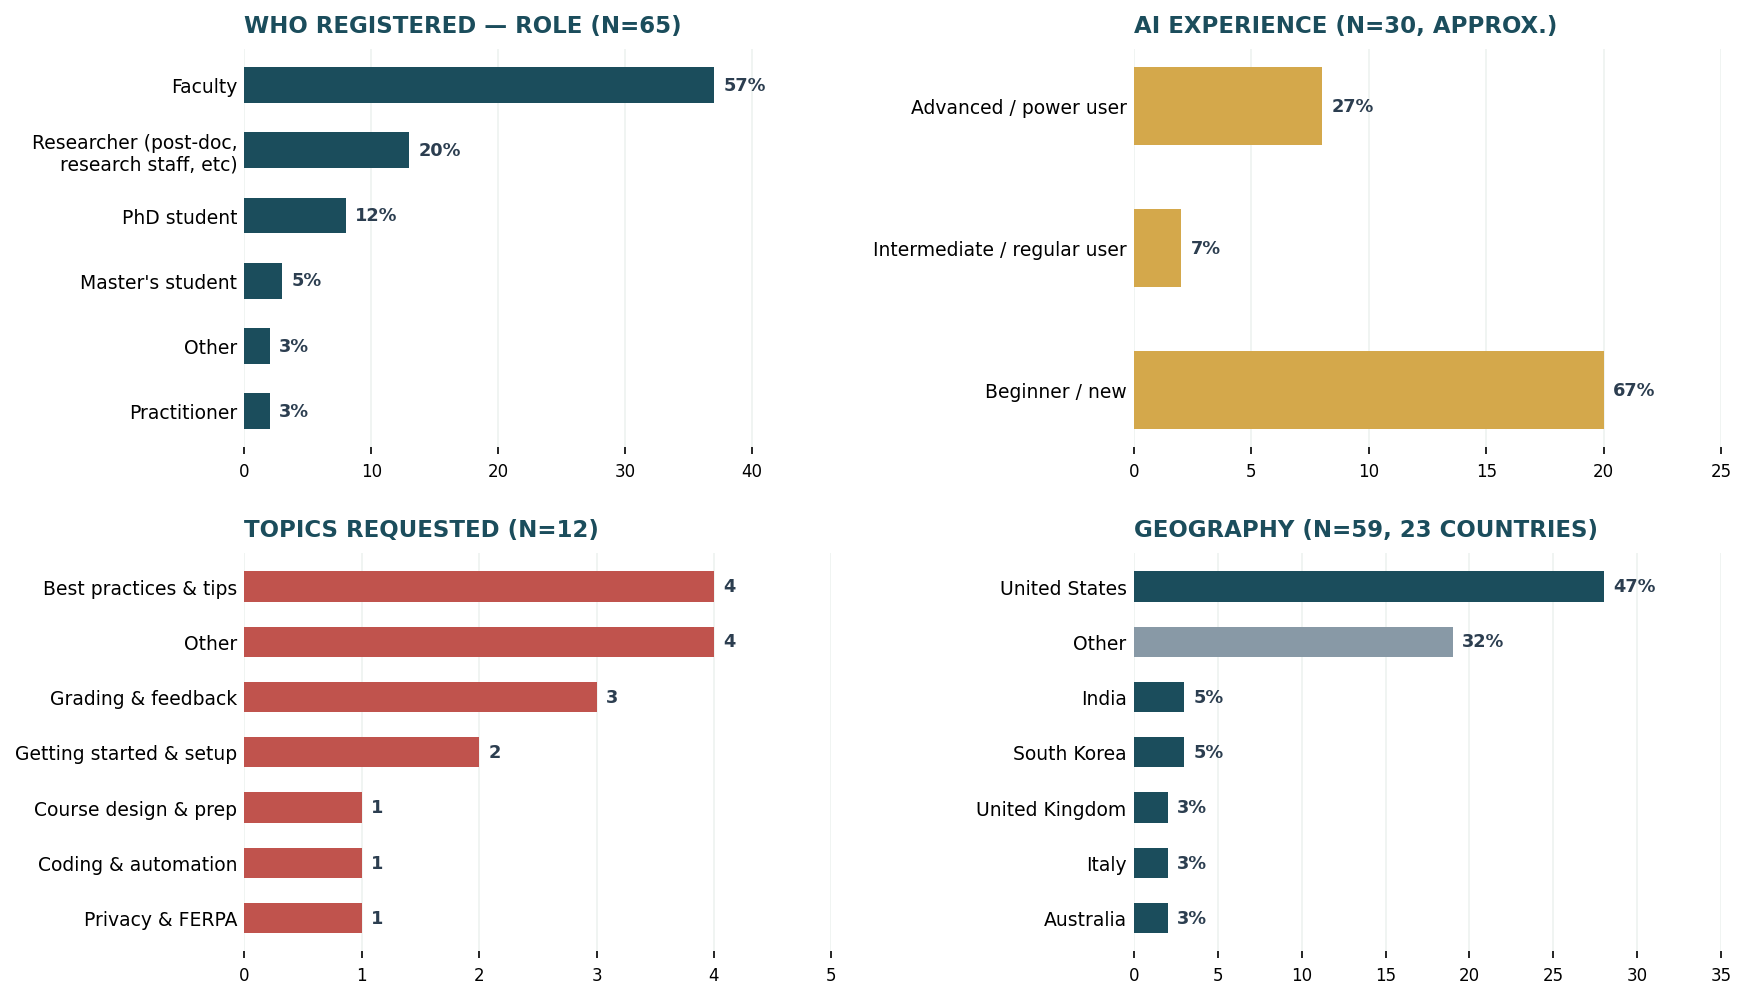
\includegraphics[width=0.90\textwidth, height=0.74\textheight, keepaspectratio]{audience_charts_teaching.png}
\end{center}
\end{frame}

%% ====== TODAY'S ARC ======
\begin{frame}{Today's plan}
\vskip2pt
\begin{columns}[T]
\begin{column}{0.48\textwidth}
\begin{tcolorbox}[keybox, title={\faLock\quad Hour 1: Emily --- grading}]
\small
\begin{itemize}\setlength{\itemsep}{4pt}
	\item \textbf{Agentic Overview}: what is even happening
  \item \textbf{Student data \& AI:} what you can and can't feed a model
  \item \textbf{De-id in practice:} a live grading pipeline that never sees a student's name
\end{itemize}
\end{tcolorbox}
\end{column}
\begin{column}{0.48\textwidth}
\begin{tcolorbox}[keybox, title={\faBook\quad Hour 2: Erkmen --- teaching prep}]
\small
\begin{itemize}\setlength{\itemsep}{4pt}
  \item \textbf{Teaching prep is production} --- agents make it cheap
  \item \textbf{Lecture Builder:} papers in $\rightarrow$ notes + slides + exams out
  \item \textbf{LMS dashboards:} one prompt $\rightarrow$ interactive tool your students use
\end{itemize}
\end{tcolorbox}
\end{column}
\end{columns}
\end{frame}

%% ====== FOUNDATIONS (~10-15 min) ======
%% ---- Three ways to interact: chat / IDE / agent ----
\begin{frame}{Three ways to work with AI}
\vskip2pt
\begin{columns}[T]
\begin{column}{0.31\textwidth}
\begin{tcolorbox}[colback=PaleSage, colframe=CoolGray, boxrule=0.6pt, arc=3pt, left=5pt, right=5pt, top=3pt, bottom=3pt, title={\faComments\quad 1. Chat window}, fonttitle=\bfseries\scriptsize, coltitle=DeepCharcoal, colbacktitle=PaleSage!80]
\scriptsize
{\color{CoolGray}\textit{ChatGPT / Claude web}}
\vskip3pt
\begin{itemize}\setlength{\itemsep}{1pt}
  \item Ask questions, paste text
  \item Can write code, make outputs
  \item[\color{SoftCoral}\faTimes] Can't see your files
\end{itemize}
\vskip2pt
{\color{CoolGray} Like \textbf{texting a smart friend}.}
\end{tcolorbox}
\end{column}
\begin{column}{0.31\textwidth}
\begin{tcolorbox}[colback=PaleSage, colframe=CoolGray, boxrule=0.6pt, arc=3pt, left=5pt, right=5pt, top=3pt, bottom=3pt, title={\faCode\quad 2. In your editor}, fonttitle=\bfseries\scriptsize, coltitle=DeepCharcoal, colbacktitle=PaleSage!80]
\scriptsize
{\color{CoolGray}\textit{VS Code / Cursor}}
\vskip3pt
\begin{itemize}\setlength{\itemsep}{1pt}
  \item AI inside your coding environment
  \item Sees the file you're in
  \item Autocomplete \& inline edits
\end{itemize}
\vskip2pt
{\color{CoolGray} Like a \textbf{co-pilot} as you type.}
\end{tcolorbox}
\end{column}
\begin{column}{0.34\textwidth}
\begin{tcolorbox}[colback=LightGold, colframe=UVMGold, boxrule=0.9pt, arc=3pt, left=5pt, right=5pt, top=3pt, bottom=3pt, title={\faTerminal\quad 3. Agent}, fonttitle=\bfseries\scriptsize, coltitle=DeepCharcoal, colbacktitle=LightGold!80]
\scriptsize
{\color{SlateTeal}\textit{Claude Code / Codex}}
\vskip3pt
\begin{itemize}\setlength{\itemsep}{1pt}
  \item[\color{SlateTeal}\faCheck] Reads \& edits your files
  \item[\color{SlateTeal}\faCheck] Runs commands
  \item[\color{SlateTeal}\faCheck] Works across a project
\end{itemize}
\vskip2pt
{\color{CoolGray} Like an \textbf{RA sitting next to you} with unlimited caffeine.}
\end{tcolorbox}
\end{column}
\end{columns}
\vskip4pt
{\centering\scriptsize\color{CoolGray} The agent runs two ways: in your \textbf{terminal} (type \texttt{claude} / \texttt{codex}) or a \textbf{desktop app} --- terminal gets new features first; the app is friendlier to start.\par}
\vskip4pt
\begin{tcolorbox}[accentbox, halign=center, top=3pt, bottom=3pt]
\small Today we're focusing on \textbf{agent-based}, because it's the biggest mindset/workflow shift.
\end{tcolorbox}
\end{frame}

%% ---- Key vocabulary ----
\begin{frame}{A few terms we'll use}
\vskip4pt
\begin{center}
{\small
\renewcommand{\arraystretch}{1.35}
\begin{tabular}{>{\bfseries\raggedright\arraybackslash}m{3.0cm} >{\raggedright\arraybackslash}m{9.6cm}}
\rowcolor{SlateTeal}
\textcolor{white}{\textbf{Term}} & \textcolor{white}{\textbf{What we mean}} \\
\rowcolor{PaleSage}
Model & The underlying AI system (e.g., Claude Sonnet, GPT-5) \\
\rowcolor{white}
Token & The unit AI models process --- roughly $\frac{3}{4}$ of a word \\
\rowcolor{PaleSage}
Session & One conversation or working thread with the tool \\
\rowcolor{white}
Context window & The working memory of the current session  \\
\rowcolor{PaleSage}
Agent & A tool carrying out a bounded task with some autonomy \\
\rowcolor{white}
Artifact & A saved output you can pull back up and reuse --- a prompt, file, table, or memo \\
\end{tabular}
}
\end{center}
\end{frame}

%% ---- Getting started ----
\begin{frame}{What do you need to get started?}
\vskip8pt
\begin{itemize}\setlength{\itemsep}{6pt}
  \item \textbf{A paid subscription}: \$20/mo Claude Pro or ChatGPT Plus will be enough to get started!
  \vspace{-2pt}
  \begin{itemize}\setlength{\itemsep}{1pt}
    \item In general, ChatGPT (currently) subscriptions yield more usage/\$
    \item Heavier users upgrade to \$100/mo or \$200/mo subscriptions
  \end{itemize}
  \item \textbf{Terminal or AI desktop app (Claude or Codex)} --- or both!
\end{itemize}
\vskip8pt
\begin{center}\begin{tcolorbox}[accentbox, halign=center, width=8cm, top=2pt, bottom=2pt]
\small\bfseries https://thinkingwithagents.github.io/install.html
\end{tcolorbox}\end{center}
\end{frame}

%% ---- Chatbot vs. agent ----
\begin{frame}{Chatbot vs. agent}
\vskip2pt
\begin{columns}[T]
\begin{column}{0.46\textwidth}
\begin{tcolorbox}[dontbox, title={\faComments\quad A chatbot}]
\small
\begin{itemize}\setlength{\itemsep}{2pt}
  \item You type a message, it replies
  \item You copy the output somewhere
  \item It has no idea what's on your computer
  \item Each turn starts fresh
\end{itemize}
\end{tcolorbox}
\end{column}
\begin{column}{0.50\textwidth}
\begin{tcolorbox}[dobox, title={\faRobot\quad An agent}]
\small
\begin{itemize}\setlength{\itemsep}{2pt}
  \item \textbf{Reads your actual files} --- papers, code, data dictionaries
  \item \textbf{Runs commands} --- Stata, Python, LaTeX, git
  \item \textbf{Remembers across turns} --- standing instructions, project context
  \item Asks permission before doing anything risky
\end{itemize}
\end{tcolorbox}
\end{column}
\end{columns}
\vskip4pt
\begin{tcolorbox}[accentbox, top=2pt, bottom=2pt]
\small
The agent's advantage isn't intelligence --- it's \textbf{context}. It sees your files, your project structure, your conventions. That's what makes it useful for real teaching work, not just one-off questions.
\end{tcolorbox}
\end{frame}

%% ---- Scope of access / sandboxing ----
\begin{frame}{What it can touch --- and how you widen it}
\vskip2pt
\begin{columns}[T,onlytextwidth]
\begin{column}{0.32\textwidth}
\begin{tcolorbox}[colback=PaleSage, colframe=SlateTeal, boxrule=0.9pt, arc=3pt, left=5pt, right=5pt, top=3pt, bottom=3pt, title={\faFolderOpen\quad 1. Default}, fonttitle=\bfseries\small\color{white}, coltitle=white, colbacktitle=SlateTeal]
\footnotesize
\textbf{Your working directory only.}
\vskip2pt
Asks before each action. Where you start, and where most work happens.
\end{tcolorbox}
\end{column}
\begin{column}{0.32\textwidth}
\begin{tcolorbox}[colback=LightGold, colframe=UVMGold, boxrule=0.9pt, arc=3pt, left=5pt, right=5pt, top=3pt, bottom=3pt, title={\faKey\quad 2. Widen}, fonttitle=\bfseries\small\color{white}, coltitle=white, colbacktitle=UVMGold]
\footnotesize
\textbf{Grant more as trust grows.}
\vskip2pt
More folders, standing permissions for actions you've vetted --- loosened deliberately.
\end{tcolorbox}
\end{column}
\begin{column}{0.32\textwidth}
\begin{tcolorbox}[colback=PaleSage, colframe=CoolGray, boxrule=0.9pt, arc=3pt, left=5pt, right=5pt, top=3pt, bottom=3pt, title={\faServer\quad 3. Sandbox / VM}, fonttitle=\bfseries\small\color{white}, coltitle=white, colbacktitle=CoolGray]
\footnotesize
\textbf{Isolated environment.}
\vskip2pt
For big, autonomous jobs --- it runs freely in a space that \emph{can't} touch the rest of your machine.
\end{tcolorbox}
\end{column}
\end{columns}
\vfill
\begin{tcolorbox}[accentbox, top=2pt, bottom=2pt]
\scriptsize Real isolation: run the agent in a sandbox using Docker, virtual environment, or other tools --- free rein inside a container that can't touch your machine.
\end{tcolorbox}
\end{frame}

%% ============================================================
%% PART 1: STUDENT DATA AND AI
%% ============================================================

{
\setbeamertemplate{footline}{}
\setbeamercolor{background canvas}{bg=SlateTeal}
\begin{frame}[plain, noframenumbering]
\centering\vfill
{\fontsize{22}{28}\bfseries\selectfont\color{white} Part 1}\\[6pt]
{\color{UVMGold}\rule{5cm}{0.8pt}}\\[6pt]
{\normalsize\color{UVMGold} Student Data and AI}\\[4pt]
{\small\color{PaleSage} What you can --- and can't --- feed a model}
\vfill
\end{frame}
}

%% ====== SLIDE: THE 30-SECOND VERSION ======
\begin{frame}{The 30-second version}
\vskip-4pt
\begin{tcolorbox}[accentbox, top=1pt, bottom=1pt]
\footnotesize
\textbf{Every country has rules about student data.} The moment you put identifiable student work into an AI tool, those rules apply. The details vary --- FERPA (US), GDPR (EU), POPIA (South Africa), PDPA (Asia-Pacific) --- but the logic is the same everywhere.
\end{tcolorbox}
\vskip1pt
\begin{columns}[T]
\begin{column}{0.48\textwidth}
\begin{tcolorbox}[dobox, title={\faCheck\quad Path 1: Approved tool}, top=1pt, bottom=1pt]
\footnotesize Use an AI tool your \textbf{institution has vetted and contracted} --- under institutional control, with a data-processing agreement.
\end{tcolorbox}
\end{column}
\begin{column}{0.48\textwidth}
\begin{tcolorbox}[dobox, title={\faCheck\quad Path 2: De-identify}, top=1pt, bottom=1pt]
\footnotesize \textbf{Properly de-identify} the data first, so it's no longer protected information. Then use any tool.
\end{tcolorbox}
\end{column}
\end{columns}
\vskip2pt
\begin{tcolorbox}[dontbox, title={\faBan\quad The universal don't}, top=1pt, bottom=1pt]
\footnotesize Never paste identifiable student work or grades into a \textbf{personal/consumer} AI account. That's a disclosure your institution hasn't authorized.
\end{tcolorbox}
\vskip1pt
\cmcite{US examples reference FERPA (34 CFR Part 99); principles generalize across frameworks. Not legal advice --- defer to your institution's policy.}
\end{frame}

%% ====== SLIDE: WHAT COUNTS AS IDENTIFIABLE ======
\begin{frame}{What counts as identifiable student data}
\vskip-2pt
\begin{columns}[T]
\begin{column}{0.50\textwidth}
\begin{tcolorbox}[keybox, title={\faLock\quad Student data protection laws cover\ldots}, top=2pt, bottom=2pt]
\small
\begin{itemize}\setlength{\itemsep}{1pt}
  \item Grades, transcripts, class lists, student work
  \item Records \textbf{held by a vendor on your behalf} (they stay protected after handoff)
  \item \textbf{Direct} identifiers (name, ID, email)
  \item \textbf{Indirect} identifiers (DOB, writing style, topic)
\end{itemize}
\vskip2pt
\footnotesize The test: could a reasonable person in your community identify the student? If yes, it's identifiable.
\end{tcolorbox}
\end{column}
\begin{column}{0.46\textwidth}
\begin{tcolorbox}[coralbox, title={\faExclamationTriangle\quad The mosaic effect}, top=2pt, bottom=2pt]
\small
In a \textbf{small seminar}, an ``anonymized'' essay can still be re-identifiable from:
\vskip2pt
\begin{itemize}\setlength{\itemsep}{1pt}
  \item topic choice
  \item writing style
  \item facts you already know about the student
\end{itemize}
\vskip2pt
De-identification means addressing \textbf{combinations} --- not just deleting the name.
\end{tcolorbox}
\vskip3pt
\begin{tcolorbox}[quotebox, top=2pt, bottom=2pt]
\scriptsize A \emph{student} pasting their \emph{own} work into a consumer tool is their choice. The obligation runs to \textbf{you and the institution}.
\end{tcolorbox}
\end{column}
\end{columns}
\end{frame}

%% ====== SLIDE: WHAT PATH 1 LOOKS LIKE ======
\begin{frame}{What Path 1 actually looks like across US institutions}
\vskip-8pt
\begin{center}
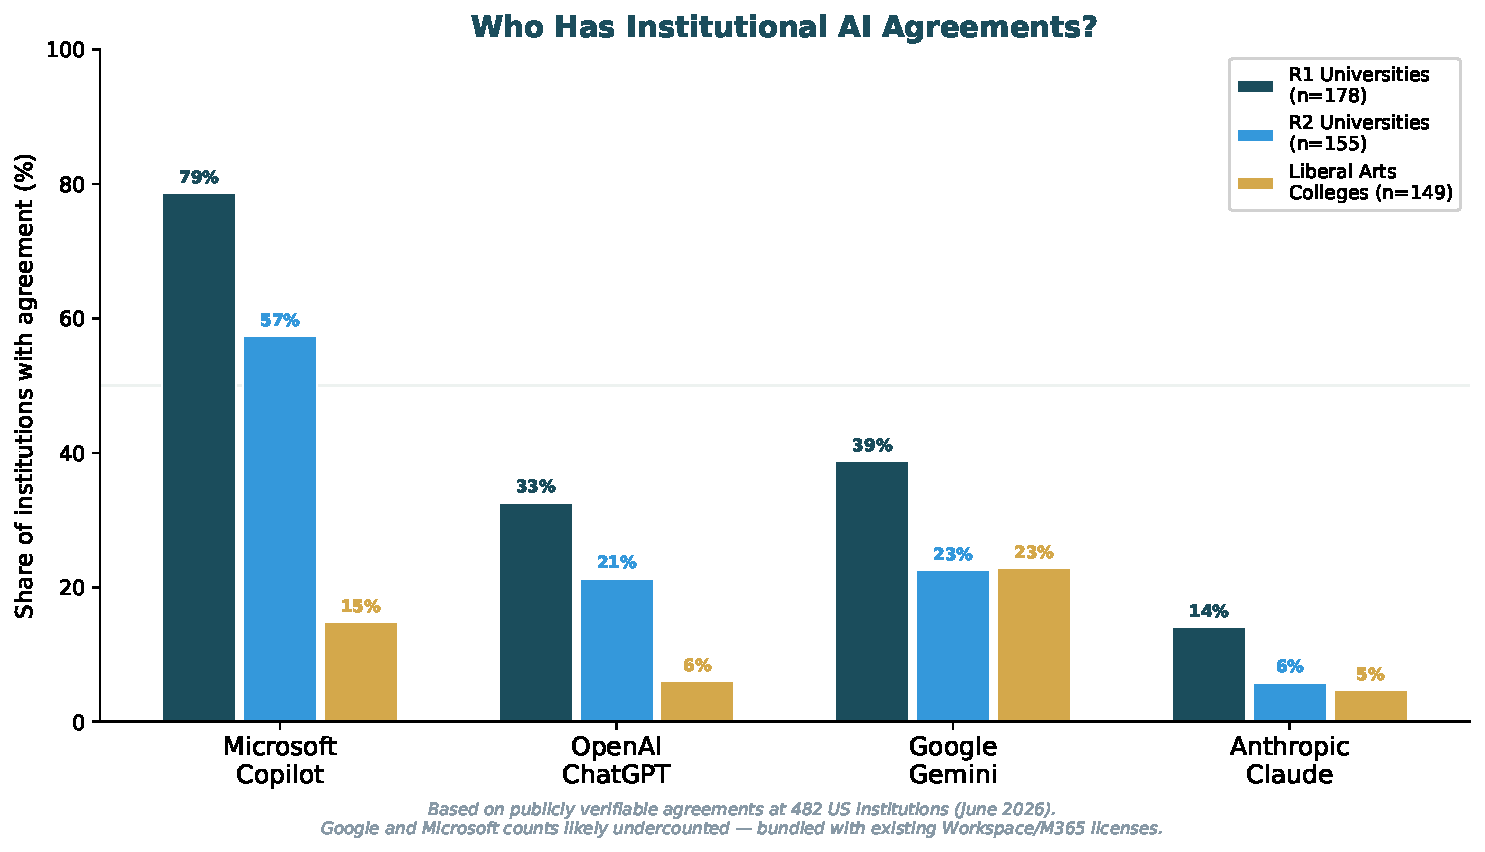
\includegraphics[width=0.86\textwidth, height=0.64\textheight, keepaspectratio]{vendor_coverage.pdf}
\end{center}
\vskip-4pt
\begin{tcolorbox}[accentbox, top=1pt, bottom=1pt]
\centering\footnotesize If your institution hasn't contracted an AI tool, \textbf{Path 2 (de-identify) is your only clean option.}
\end{tcolorbox}
\end{frame}

%% ====== SLIDE: SCENARIOS ======
\begin{frame}{Concrete classroom scenarios}
\vskip-2pt
{\small
\begin{tabular}{>{\raggedright\arraybackslash}m{7.3cm} >{\centering\arraybackslash}m{1.3cm} >{\raggedright\arraybackslash}m{3.4cm}}
\rowcolor{SlateTeal}
\textcolor{white}{\textbf{Scenario}} & \textcolor{white}{\textbf{Verdict}} & \textcolor{white}{\textbf{Why}} \\[2pt]
\rowcolor{PaleSage}
Named essay into consumer ChatGPT for feedback & \textcolor{SoftCoral}{\faTimes} & Unconsented disclosure \\[3pt]
\rowcolor{white}
Same essay, \textbf{fully de-identified}, low re-ID risk, general tool & \textcolor{UVMGold}{\faExclamationTriangle} & Defensible --- your judgment \\[3pt]
\rowcolor{PaleSage}
Same essay, in the \textbf{university's contracted} tool & \textcolor{GoGreen}{\faCheck} & Vendor is a school official \\[3pt]
\rowcolor{white}
Upload the class gradebook to summarize performance & \textcolor{SoftCoral}{\faTimes} & Grades are PII \\[3pt]
\rowcolor{PaleSage}
Course chatbot \textbf{trained on} student submissions & \textcolor{SoftCoral}{\faTimes} & Needs approval + DPA \\[3pt]
\rowcolor{white}
AI to draft a \textbf{generic} rubric or lecture (no student data) & \textcolor{GoGreen}{\faCheck} & No education records involved \\[2pt]
\end{tabular}
}
\vskip5pt
\begin{tcolorbox}[quotebox, width=12.5cm, top=3pt, bottom=3pt]
\small The dividing line is almost always: \textbf{identifiable student data + a tool that isn't institutionally controlled.}
\end{tcolorbox}
\end{frame}

%% ============================================================
%% PART 2: DE-IDENTIFICATION IN PRACTICE
%% ============================================================

{
\setbeamertemplate{footline}{}
\setbeamercolor{background canvas}{bg=SlateTeal}
\begin{frame}[plain, noframenumbering]
\centering\vfill
{\fontsize{22}{28}\bfseries\selectfont\color{white} Part 2}\\[6pt]
{\color{UVMGold}\rule{5cm}{0.8pt}}\\[6pt]
{\normalsize\color{UVMGold} De-Identification in Practice}\\[4pt]
{\small\color{PaleSage} A live grading pipeline that never sees a student's name}
\vfill
\end{frame}
}

%% ====== SLIDE: THE ASSIGNMENT ======
\begin{frame}{The assignment I want to grade}
\vskip-8pt
\begin{center}
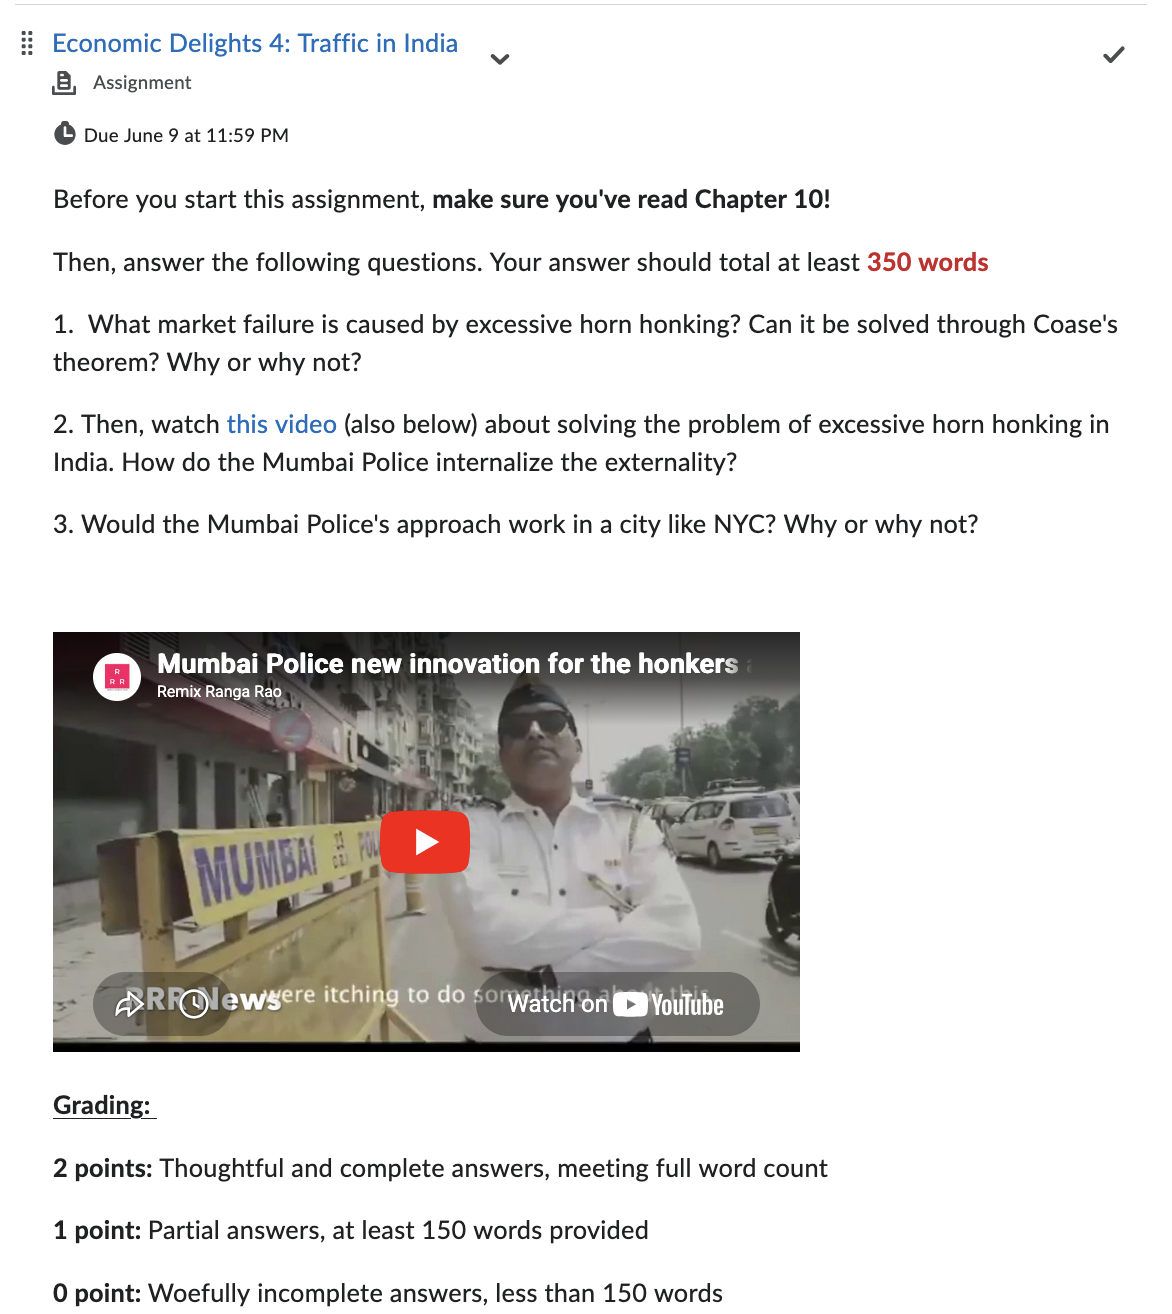
\includegraphics[width=0.75\textwidth, height=0.78\textheight, keepaspectratio]{ed4_assignment.png}
\end{center}
\end{frame}

%% ====== SLIDE: DECISION FLOW ======
\begin{frame}{The decision flow: student work $\rightarrow$ AI}
\vskip-2pt
\begin{center}
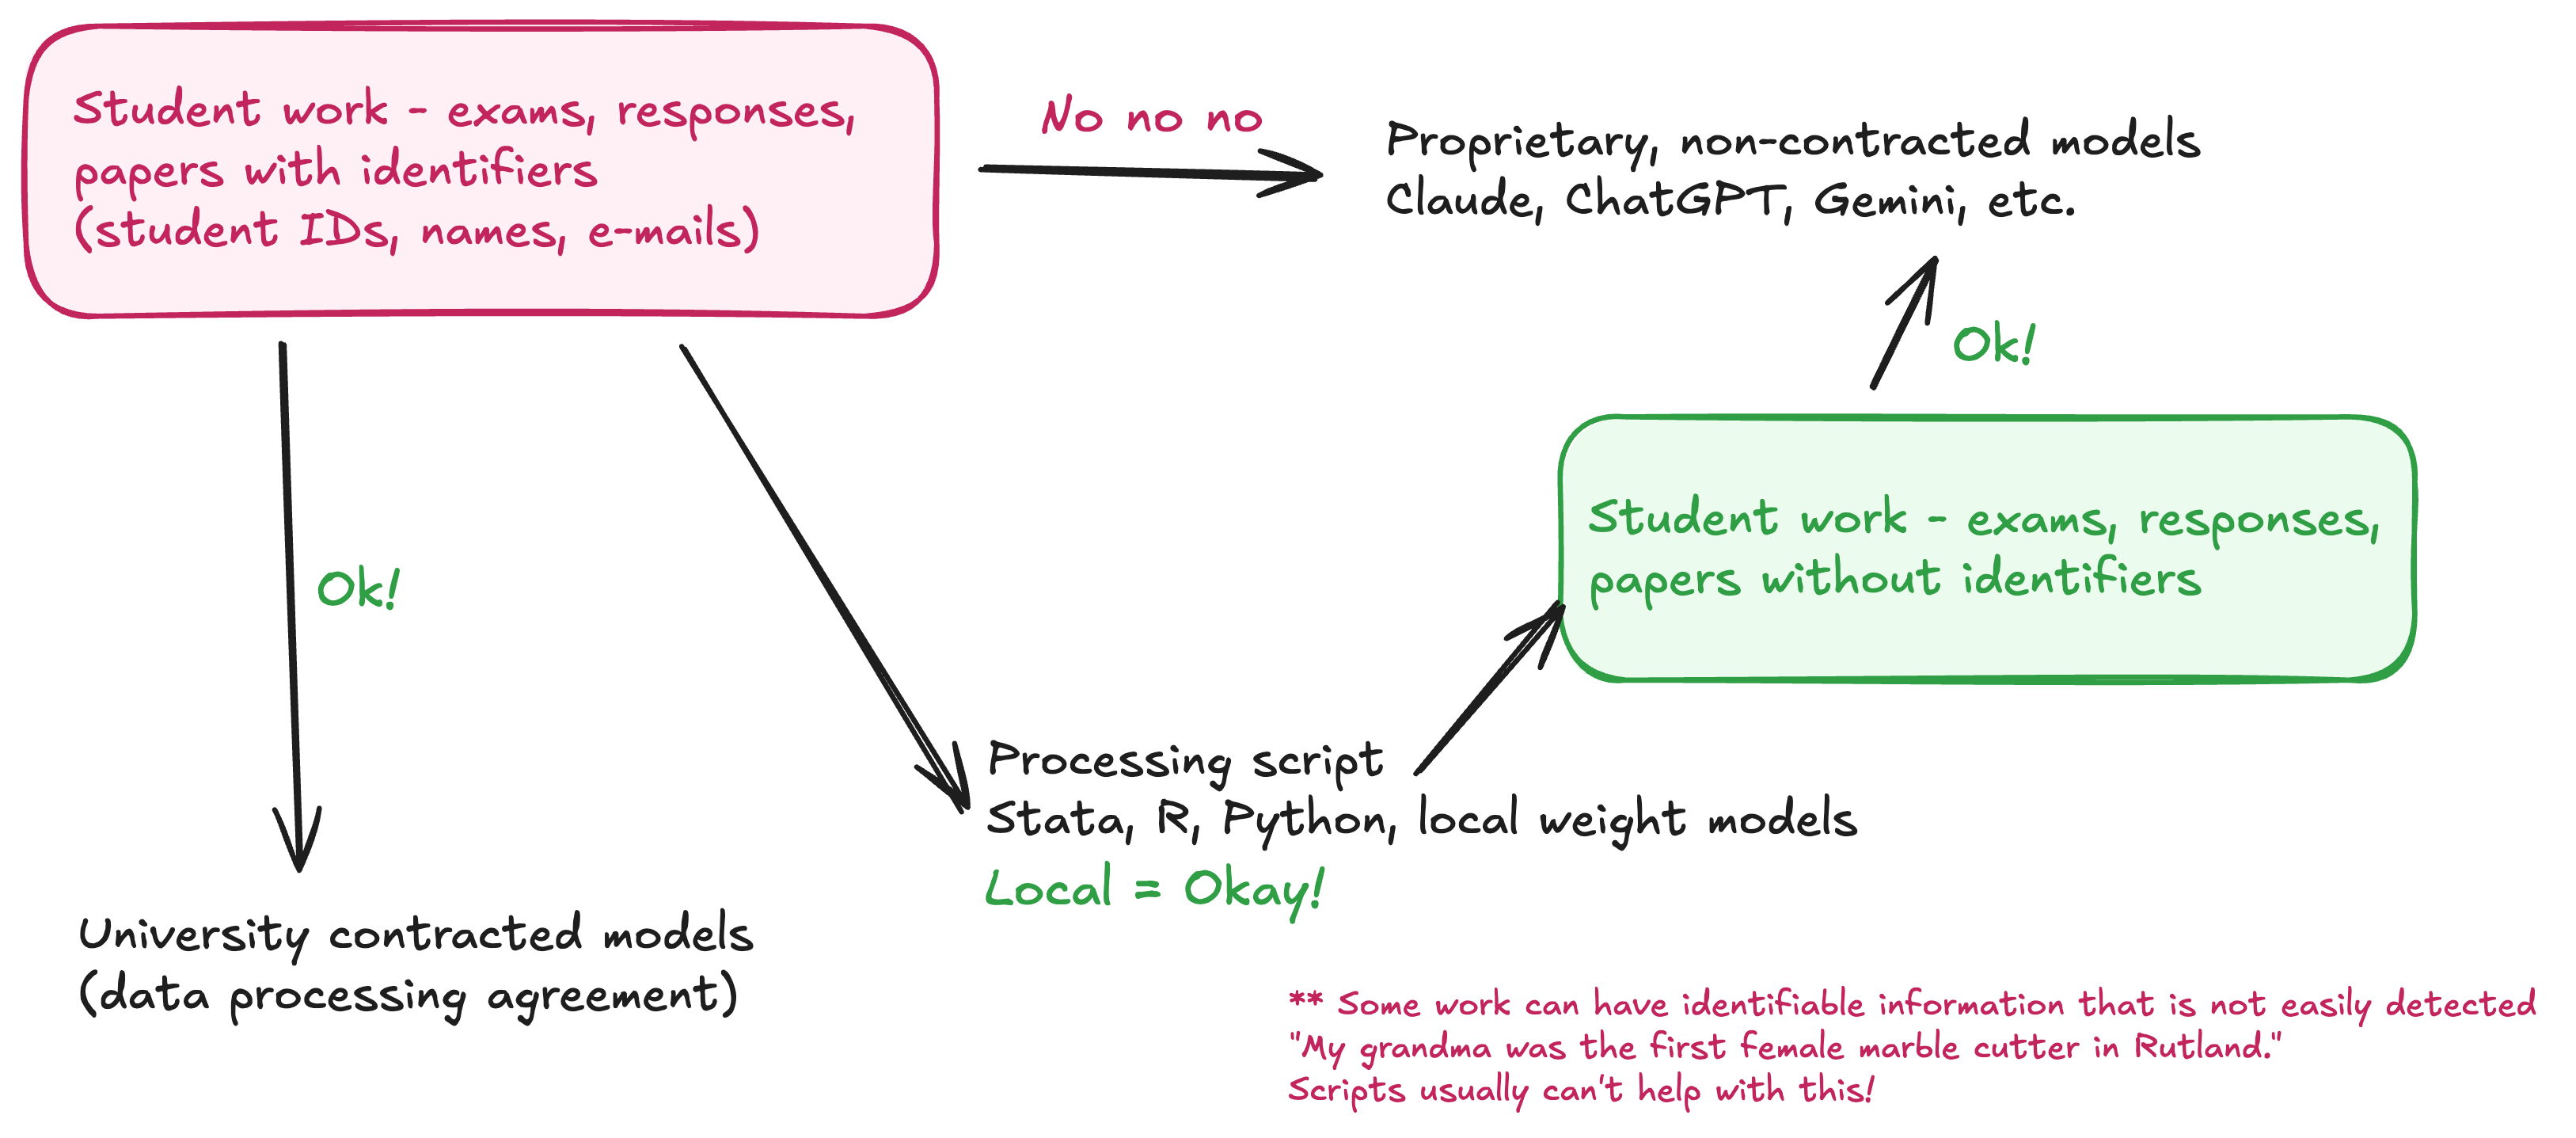
\includegraphics[width=0.92\textwidth]{ferpa-student-work-decision-flow.png}
\end{center}
\vskip2pt
{\scriptsize\color{CoolGray} Some student work has identifiable \emph{content} that isn't a named entity --- e.g., ``My grandma was the first female marble cutter in Rutland.'' Scripts strip names and IDs; they can't catch this. For these cases, route to a contracted tool instead.\par}
\end{frame}

%% ====== SLIDE: BRIDGE ======
\begin{frame}{A grading pipeline}
\vskip4pt
\begin{tcolorbox}[accentbox, top=4pt, bottom=4pt]
\small Path 2 says: \textbf{de-identify first, then use any tool you want.} \\[4pt]
What does that actually look like for the most common task --- \textbf{grading essays at scale}?
\end{tcolorbox}
\vskip8pt
\begin{tcolorbox}[dobox, title={\faCheck\quad What a pipeline enables}]
\small
\begin{itemize}\setlength{\itemsep}{3pt}
  \item \textbf{Strip PII automatically} before any AI sees the work
  \item Run a \textbf{rubric-driven agent} on anonymous text
  \item \textbf{Your review} catches edge cases and flags
  \item Export a \textbf{grade CSV} straight to your LMS
\end{itemize}
\end{tcolorbox}
\end{frame}

%% ====== SLIDE: THE PIPELINE ======
\begin{frame}{The pipeline}
\vskip-4pt
\begin{center}
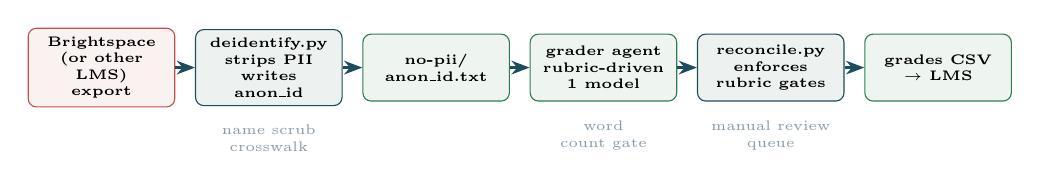
\begin{tikzpicture}[
  node distance=0.4cm and 0.25cm,
  box/.style={rectangle, rounded corners=3pt, draw=SlateTeal, fill=PaleSage,
    text width=1.65cm, align=center, font=\tiny\bfseries, minimum height=0.85cm,
    inner sep=3pt},
  piibox/.style={rectangle, rounded corners=3pt, draw=SoftCoral, fill=SoftCoral!8,
    text width=1.65cm, align=center, font=\tiny\bfseries, minimum height=0.85cm,
    inner sep=3pt},
  safenode/.style={rectangle, rounded corners=3pt, draw=GoGreen, fill=GoGreen!8,
    text width=1.65cm, align=center, font=\tiny\bfseries, minimum height=0.85cm,
    inner sep=3pt},
  arr/.style={-Stealth, thick, color=SlateTeal},
  label/.style={font=\tiny\color{CoolGray}, align=center, text width=1.65cm}
]
  \node[piibox] (bs)   {Brightspace\\(or other LMS)\\export};
  \node[box, right=of bs] (deid)  {deidentify.py\\strips PII\\writes anon\_id};
  \node[safenode, right=of deid] (nopii) {no-pii/\\anon\_id.txt};
  \node[safenode, right=of nopii] (agent) {grader agent\\rubric-driven\\1 model};
  \node[box, right=of agent] (rec)  {reconcile.py\\enforces\\rubric gates};
  \node[safenode, right=of rec] (csv)  {grades CSV\\$\rightarrow$ LMS};

  \draw[arr] (bs) -- (deid);
  \draw[arr] (deid) -- (nopii);
  \draw[arr] (nopii) -- (agent);
  \draw[arr] (agent) -- (rec);
  \draw[arr] (rec) -- (csv);

  \node[label, below=0.12cm of deid] {name scrub\\crosswalk};
  \node[label, below=0.12cm of agent] {word count gate};
  \node[label, below=0.12cm of rec]  {manual review\\queue};
\end{tikzpicture}
\end{center}
\vskip3pt
\begin{tcolorbox}[accentbox, top=2pt, bottom=2pt]
\centering\small \textbf{At no point does the AI see a name, student ID, or anything that re-identifies the student.}
\end{tcolorbox}
\vskip2pt
\begin{columns}[T]
\begin{column}{0.48\textwidth}
\begin{tcolorbox}[pipelinebox, title={\faLock\quad PII stays locked}]
\scriptsize
Filenames $\rightarrow$ crosswalk $\rightarrow$ \texttt{anon\_id}. \\
Student names scrubbed from text. \\
\texttt{pii/} folder never sent to agent.
\end{tcolorbox}
\end{column}
\begin{column}{0.48\textwidth}
\begin{tcolorbox}[pipelinebox, title={\faFileCode\quad Any submission format}]
\scriptsize
Handles HTML text-box, DOCX, and PDF --- all three formats Brightspace produces.
\end{tcolorbox}
\end{column}
\end{columns}
\end{frame}


%% ====== SLIDE: PII GUARDRAIL ======
\begin{frame}{My PII guardrail: what I actually use}
\vskip-4pt
\begin{tcolorbox}[accentbox, top=1pt, bottom=1pt]
\footnotesize I asked the agent to write a \textbf{pre-tool hook} --- a shell script that fires automatically before every file read or terminal command. It took about 30 seconds. I've been refining it since.
\end{tcolorbox}
\vskip2pt
\begin{columns}[T]
\begin{column}{0.48\textwidth}
\begin{tcolorbox}[pipelinebox, title={\faLock\quad What it blocks}, top=2pt, bottom=2pt]
\footnotesize
\begin{itemize}\setlength{\itemsep}{1pt}
  \item \textbf{Read tool}: data/geo files (\texttt{.csv}, \texttt{.dta}, \texttt{.sav}, \texttt{.shp}, \texttt{.parquet}, etc.)
  \item \textbf{Bash dumps}: \texttt{cat}, \texttt{head}, \texttt{grep}, \texttt{awk} on data files
  \item \textbf{Protected folders}: paths where even non-data files contain PII
  \item \textbf{LMS exports}: detects Brightspace/Canvas folder-name patterns where student names are baked into subfolder titles
\end{itemize}
\end{tcolorbox}
\end{column}
\begin{column}{0.48\textwidth}
\begin{tcolorbox}[pipelinebox, title={\faCheck\quad What it allows}, top=2pt, bottom=2pt]
\footnotesize
\begin{itemize}\setlength{\itemsep}{1pt}
  \item \texttt{python3 script.py} --- scripts read PII, write outputs to disk, print only \textbf{aggregates}
  \item \textbf{Schema inspection}: column names and types, no values
  \item \textbf{Per-project unlock}: add a folder to \texttt{SAFE\_PATHS} to mark it PII-free
\end{itemize}
\vskip3pt
\begin{tcolorbox}[accentbox, top=1pt, bottom=1pt]
\scriptsize \textbf{The principle}: a script may read PII; the agent context must never see raw PII rows.
\end{tcolorbox}
\end{tcolorbox}
\end{column}
\end{columns}
\end{frame}



%% ====== SLIDE: LIVE DEMO ======
{
\setbeamertemplate{footline}{}
\setbeamercolor{background canvas}{bg=DarkSlate}
\begin{frame}[plain]
\centering\vfill
{\fontsize{20}{26}\bfseries\selectfont\color{white} \faTerminal\quad Live Demo}\\[10pt]
{\color{UVMGold}\rule{6cm}{0.8pt}}\\[10pt]
{\normalsize\color{PaleSage} 3 anonymized submissions \;$\cdot$\; economic-delights rubric}\\[4pt]
{\small\color{CoolGray} deidentify $\rightarrow$ count words $\rightarrow$ grade $\rightarrow$ reconcile $\rightarrow$ CSV}
\vfill
\end{frame}
}

%% ====== SLIDE: WHAT THE AGENT SEES AND WHAT STAYS YOURS ======
\begin{frame}{What the agent sees --- and what stays yours}
\vskip2pt
\begin{columns}[T]
\begin{column}{0.48\textwidth}
\begin{tcolorbox}[pipelinebox, title={\faEye\quad The agent receives}]
\scriptsize
\texttt{anon\_id: STU04}\\
\texttt{Question 1: Describe the economic tradeoff\ldots}\\
\texttt{Student response: The opportunity cost\ldots [391 words]}\\[3pt]
No name. No student ID. No course section.
\end{tcolorbox}
\vskip3pt
\begin{tcolorbox}[pipelinebox, title={\faBrain\quad The agent returns}]
\scriptsize
\begin{itemize}\setlength{\itemsep}{1pt}
  \item \textbf{Score} (0 / 1 / 2 per rubric)
  \item \textbf{Justification} (1--2 sentences)
  \item \textbf{Review queue}: flag if borderline
\end{itemize}
\end{tcolorbox}
\end{column}
\begin{column}{0.48\textwidth}
\begin{tcolorbox}[keybox, title={\faUserCheck\quad Your judgment}]
\scriptsize
\begin{itemize}\setlength{\itemsep}{2pt}
  \item \textbf{Edge cases}: embedded links, borderline word counts
  \item \textbf{Rubric calls}: you set the rubric, review anything the explanation doesn't support
  \item \textbf{Final sign-off}: grade CSV is yours before upload
\end{itemize}
\end{tcolorbox}
\vskip3pt
\begin{tcolorbox}[accentbox, top=3pt, bottom=3pt]
\scriptsize
The pipeline handles \textbf{mechanical work at scale}. \textbf{Pedagogical judgment} --- what counts as thoughtful, what warrants a flag --- is \textbf{still yours}.
\end{tcolorbox}
\end{column}
\end{columns}
\end{frame}

%% ====== SLIDE: THE REUSE PRINCIPLE ======
\begin{frame}{Built once, used every semester}
\vskip2pt
\begin{tcolorbox}[keybox, title={\faCog\quad To reuse for the next assignment}]
\small
\begin{enumerate}\setlength{\itemsep}{2pt}
  \item Copy the scripts to the new assignment's grading folder
  \item Update the \textbf{rubric YAML} (questions, thresholds, score levels)
  \item Point \texttt{DOWNLOAD\_DIR} at the new Brightspace export
  \item Run: \texttt{deid} $\rightarrow$ \texttt{count\_words} $\rightarrow$ \texttt{grade} $\rightarrow$ \texttt{reconcile}
\end{enumerate}
\end{tcolorbox}
\vskip4pt
\begin{columns}[T]
\begin{column}{0.48\textwidth}
\begin{tcolorbox}[quotebox, top=3pt, bottom=3pt]
\small
\textbf{This session's run}: ED4 (Coase theorem), 18 submissions. 16 auto-graded in $\sim$4 min. 1 manual flag, 1 embedded-doc gotcha.
\end{tcolorbox}
\end{column}
\begin{column}{0.48\textwidth}
\begin{tcolorbox}[accentbox, top=3pt, bottom=3pt]
\small
\textbf{Don't want to build it?} Describe your rubric and export format to the agent --- it writes the scripts for you.
\end{tcolorbox}
\end{column}
\end{columns}
\end{frame}


%% ====== SLIDE: EXTENSIONS ======
\begin{frame}{Extensions: from grading to better feedback}
\vskip-2pt
\begin{tcolorbox}[accentbox, top=1pt, bottom=1pt]
\small The same pipeline that grades can also \textbf{improve what students get back}.
\end{tcolorbox}
\vskip3pt
\begin{itemize}\setlength{\itemsep}{3pt}
  \item \textbf{Literature connections}: run a search for sources related to each student's topic --- suggest 2--3 papers they should read next
  \item \textbf{Constructive feedback}: generate a paragraph of specific, rubric-anchored feedback for each submission (not just a score)
  \item \textbf{Harmonized passes}: run a second agent pass across all graded submissions to flag inconsistencies in scoring
  \item \textbf{Smarter de-identification}: open-weight PII models (e.g., OpenAI Privacy Filter, $\sim$1.5B params, Apache 2.0) run \textbf{entirely on your laptop} --- learned entity detection instead of regex, $\sim$96\% F1
\end{itemize}
\vskip4pt
\begin{tcolorbox}[quotebox, top=2pt, bottom=2pt]
\small Each of these is a separate agent step you can add to the pipeline --- or skip. The base pipeline works without them.
\end{tcolorbox}
\end{frame}

%% ============================================================
%% HANDOFF TO ERKMEN
%% ============================================================

{
\setbeamertemplate{footline}{}
\setbeamercolor{background canvas}{bg=SlateTeal}
\begin{frame}[plain, noframenumbering]
\centering\vfill
{\fontsize{20}{26}\bfseries\selectfont\color{white} Over to Erkmen}\\[8pt]
{\color{UVMGold}\rule{6cm}{0.8pt}}\\[8pt]
\begin{tcolorbox}[accentbox, width=11cm, top=4pt, bottom=4pt]
\centering\small
\textbf{This hour in one line:} know the rule (FERPA) $\cdot$ use the path (de-identify) $\cdot$ let the agent do the mechanical work $\cdot$ you own the judgment.
\end{tcolorbox}
\vskip10pt
{\normalsize\color{PaleSage} Erkmen picks up here: teaching prep, the lecture-builder, and an interactive tool your students use inside your LMS.}
\vfill
\end{frame}
}

%% ============================================================
%% REFERENCE SLIDE (backup / Q&A)
%% ============================================================

\begin{frame}{Reference: the three enterprise tools, compared}
\vskip-2pt
{\footnotesize
\begin{tabular}{>{\raggedright\arraybackslash}m{3.9cm} >{\centering\arraybackslash}m{2.7cm} >{\centering\arraybackslash}m{2.7cm} >{\centering\arraybackslash}m{2.7cm}}
\rowcolor{SlateTeal}
\textcolor{white}{\textbf{}} & \textcolor{white}{\textbf{ChatGPT Edu / Enterprise}} & \textcolor{white}{\textbf{MS 365 Copilot}} & \textcolor{white}{\textbf{Claude Edu / Enterprise}} \\[1pt]
\rowcolor{PaleSage}
Trains on your data by default? & \textcolor{GoGreen}{\textbf{No}} & \textcolor{GoGreen}{\textbf{No}} & \textcolor{GoGreen}{\textbf{No}} \\[1pt]
\rowcolor{white}
Consumer tier trains by default? & Yes (opt-out) & N/A & \textbf{Yes} since Aug 2025 \\[1pt]
\rowcolor{PaleSage}
Explicit FERPA ``school official'' language? & \textcolor{SoftCoral}{No} & \textcolor{GoGreen}{\textbf{Yes}} (99.33(a)) & \textcolor{SoftCoral}{No} (processor + DPA) \\[1pt]
\rowcolor{white}
Data Processing Addendum? & Yes & Yes (OST DPA) & Yes (auto-incl.) \\[1pt]
\rowcolor{PaleSage}
Retention & Configurable & Configurable & Until deleted (API: 30d) \\[1pt]
\rowcolor{white}
Zero-data-retention option? & Via API & --- & \textbf{API only, not chat} \\[1pt]
\end{tabular}
}
\vskip4pt
\begin{tcolorbox}[quotebox, width=13cm, top=2pt, bottom=2pt]
\scriptsize All entries are \textbf{vendor representations}, not adjudicated FERPA compliance --- terms change fast. \textbf{Microsoft} alone publishes an explicit FERPA school-official commitment; the others rely on the contract/DPA + institutional vetting. \cmcite{Sources: openai.com, learn.microsoft.com, privacy.claude.com --- as of June 2026.}
\end{tcolorbox}
\end{frame}

%% ============================================================
%% APPENDIX (backup / Q&A — not in main flow)
%% ============================================================

\appendix

%% ====== APPENDIX: WHAT ED HAS SAID ======
\begin{frame}{What the Dept of Education has --- and hasn't --- said}
\begin{columns}[T]
\begin{column}{0.50\textwidth}
\begin{tcolorbox}[keybox, title={\faGavel\quad No AI-specific rules}]
\small \textbf{No AI-specific FERPA regulations exist} (as of June 2026). The existing \textbf{technology-neutral} guidance governs AI vendors directly.
\end{tcolorbox}
\vskip4pt
\begin{tcolorbox}[quotebox, top=3pt, bottom=3pt]
\scriptsize The framework (school-official exception, direct control, data-minimization) is tech-neutral --- AI tools are just a subset of ``online educational services.''
\end{tcolorbox}
\end{column}
\begin{column}{0.46\textwidth}
\begin{tcolorbox}[accentbox]
\small
\textbf{The operative ED documents:}
\vskip3pt
\begin{itemize}\setlength{\itemsep}{2pt}
  \item Third-Party Service Providers under FERPA (2015)
  \item Online Educational Services: Requirements \& Best Practices (2014)
  \item \textbf{Model Terms of Service checklist (2016)} --- ready-made for vetting a tool's ToS
\end{itemize}
\end{tcolorbox}
\vskip3pt
\cmcite{studentprivacy.ed.gov}
\end{column}
\end{columns}
\end{frame}

%% ====== APPENDIX: ENFORCEMENT REALITY ======
\begin{frame}{So how worried should you be? The enforcement reality}
\begin{columns}[T]
\begin{column}{0.50\textwidth}
\begin{tcolorbox}[keybox, title={\faBalanceScale\quad How FERPA is enforced}, top=3pt, bottom=3pt]
\small
\begin{itemize}\setlength{\itemsep}{2pt}
  \item \textbf{No private right of action} --- a student cannot sue you under FERPA \cmcite{(\textit{Gonzaga v. Doe}, 2002)}.
  \item ED's ultimate stick is \textbf{withdrawing federal funds} --- never actually used.
  \item Real ed-tech enforcement has run through \textbf{COPPA/FTC}, not FERPA (Edmodo, \$6M, 2023).
\end{itemize}
\end{tcolorbox}
\end{column}
\begin{column}{0.46\textwidth}
\begin{tcolorbox}[accentbox]
\small
\textbf{The real exposure is institutional and reputational}, not a lawsuit.
\vskip3pt
That's exactly why your university \textbf{vets and contracts} tools centrally --- and why the safe move is to \textbf{use the approved one}.
\end{tcolorbox}
\vskip3pt
\begin{tcolorbox}[quotebox, top=2pt, bottom=2pt]
\scriptsize ED's only recent vendor action (the May 2026 Canvas/Instructure letter) was about a \textbf{data breach} --- not AI. There is still \textbf{no AI-specific FERPA guidance}.
\end{tcolorbox}
\end{column}
\end{columns}
\end{frame}

%% ====== APPENDIX: MODEL TRAINING ======
\begin{frame}{The question everyone asks: ``does it train on my data?''}
\begin{columns}[T]
\begin{column}{0.50\textwidth}
\begin{tcolorbox}[keybox, title={\faBrain\quad The FERPA answer}, top=3pt, bottom=3pt]
\small
Under the school-official exception, a vendor may use PII \textbf{only for the contracted purpose} and may not reuse it for its own ends.
\vskip3pt
So training a vendor's models on \textbf{identifiable} student records is an \textbf{unauthorized reuse} --- unless you authorize it.
\vskip3pt
\textbf{De-identified} data is outside FERPA --- training on it is fine.
\end{tcolorbox}
\vskip3pt
\cmcite{ED 2014/2016 guidance; CRS R46799. A sound inference from the use-limitation rule --- ED has no AI-specific ruling.}
\end{column}
\begin{column}{0.46\textwidth}
\begin{tcolorbox}[coralbox, title={\faExclamationTriangle\quad The vendor reality}, top=2pt, bottom=2pt]
\small
\begin{itemize}\setlength{\itemsep}{1pt}
  \item OpenAI, MS 365 Copilot, and Claude (\textbf{commercial/edu} tiers) all state they don't train on your prompts \emph{by default}.
  \item These are \textbf{vendor statements}, not FERPA rulings --- and consumer tiers are excluded.
  \item Only \textbf{Microsoft} publishes an explicit FERPA ``school-official'' commitment.
\end{itemize}
\end{tcolorbox}
\vskip3pt
\cmcite{Full three-way comparison on the reference slide.}
\end{column}
\end{columns}
\end{frame}

%% ====== COMMENTED OUT: TAKEAWAYS ======
%% \begin{frame}{Takeaways: a faculty checklist}
%% \vskip2pt
%% \begin{tcolorbox}[keybox, title={\faClipboardCheck\quad Before you put student data in any AI tool}]
%% \small
%% \begin{enumerate}\setlength{\itemsep}{4pt}
%%   \item Is it \textbf{identifiable} student data? (Remember: PII is broader than names.)
%%   \item If yes --- is the tool \textbf{institutionally vetted / contracted}? If not, \textbf{stop}.
%%   \item Or can you \textbf{properly de-identify} it (risk-based, hard in small classes)?
%%   \item When in doubt, run the ToS through ED's \textbf{Model ToS checklist} and ask your \textbf{privacy office}.
%% \end{enumerate}
%% \end{tcolorbox}
%% \vskip6pt
%% \begin{tcolorbox}[accentbox, width=12.5cm]
%% \centering\small \textbf{The one thing to remember:} approved tool \emph{or} de-identify --- never identifiable student data in a personal AI account.
%% \end{tcolorbox}
%% \end{frame}

\end{document}
